\chapter{Assignment solutions-Hamilltonian Equation of Motion}
\begin{abox}
Assignment solution-1
\end{abox}
\begin{enumerate}
	\item $\left. \right. $
	\begin{answer}
		\begin{align*}
		\text{(A) }T&=\frac{1}{2} m\left(\dot{r}^{2}+r^{2} \dot{\theta}^{2}+\dot{z}^{2}\right)=\frac{m}{2}\left(\dot{r}^{2}+r^{2} \dot{\theta}^{2}+a^{2} r^{2} \dot{r}^{2}\right) \quad \because z=\frac{1}{2} a r^{2} \Rightarrow \quad \dot{z}=a r \dot{r}\\
		V&=m g z=\frac{1}{2} m g a r^{2} \\
		L&=\frac{m}{2}\left[\dot{r}^{2}\left(1+a^{2} r^{2}\right)+r^{2} \dot{\theta}^{2}-a g r^{2}\right]
	\intertext{	(a) $\theta$ is cyclic coordinate}
	\because \frac{\partial L}{\partial \theta}&=0, \Rightarrow \dot{p}_{\theta}=0 \Rightarrow P_{\theta}=\text{ constant}
	\intertext{(b) Hamiltonian}
	H&=\frac{p_{r}^{2}}{2 m\left(1+a^{2} r^{2}\right)}+\frac{p_{\theta}^{2}}{2 m r^{2}}+\frac{1}{2} m a g r^{2} \quad \\&\because \frac{\partial L}{\partial \dot{r}}=p_{r}=m\left(1+a^{2} r^{2}\right) \dot{r}\text{ and }\frac{\partial L}{\partial \dot{\theta}}=p_{\theta}=m r^{2} \dot{\theta}
		\end{align*}
	\end{answer}
	\item $\left. \right. $
	\begin{figure}[H]
		\centering
		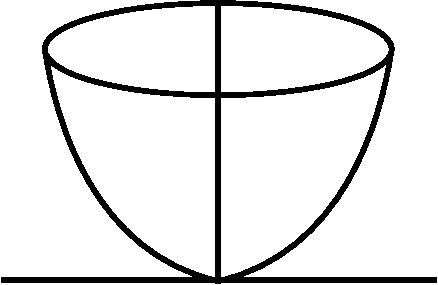
\includegraphics[height=2cm,width=3.5cm]{diagram-20220314-9-crop}
	\end{figure}
    \begin{answer}
    	\begin{align*}
    	\because z&=a\left(x^{2}+y^{2}\right)
    	\intertext{Using equation of constrain, we must solve the given system in cylindrical co-ordinate.}
    	z&=a r^{2}, \dot{z}=2 a r \dot{r}\\
    	L&=\frac{1}{2} m\left(\dot{r}^{2}+r^{2} \dot{\theta}^{2}+\dot{z}^{2}\right)-m g z\\
    	\Rightarrow L=\frac{1}{2} m\left(\dot{r}^{2}+r^{2} \dot{\theta}^{2}+4 a^{2} r^{2} \dot{r}^{2}\right)-m g a r^{2}&=\frac{1}{2} m\left(\dot{r}^{2}\left(1+4 a^{2} r^{2}\right)+r^{2} \dot{\theta}^{2}\right)-m g a r^{2}\\
    	\text{Equation of motion }&\frac{d}{d t}\left(\frac{\partial L}{\partial \dot{r}}\right)-\frac{\partial L}{\partial r}=0\\
    	m \ddot{r}\left(1+4 a^{2} r^{2}\right)&+4 m \dot{r}^{2} a^{2} r-m r \dot{\theta}^{2}+2 m g a r=0\\
    	\text{At }z=z_{0}, \quad \dot{r}&=0, \quad r=r_{0} \Rightarrow+m r_{0} \dot{\theta}^{2}=2 m g a r_{0} \Rightarrow \dot{\theta}=\sqrt{2 g a}\\
    	\Rightarrow \frac{v}{r_{0}}=\sqrt{2 g a} \Rightarrow v&=\sqrt{2 g a} \cdot r_{0}=\sqrt{2 g a} \cdot\left(\frac{z_{0}}{a}\right)^{1 / 2} \Rightarrow v=\sqrt{2 g z_{0}}\\
    	\because z_{0}&=a r_{0}^{2}
    	\end{align*}
    \end{answer}
	\item $\left. \right. $
	\begin{answer}
		\begin{align*}
		(a) x_{1}=0, x_{2}=l \sin \theta \Rightarrow \dot{x}_{2}&=l \cos \theta \dot{\theta}\\
		y_{2}=y_{1}+l \cos \theta, \quad \dot{y}_{2}&=\dot{y}_{1}-l \sin \theta \dot{\theta}\\
		L=\frac{M}{2}\left(\dot{y}_{1}^{2}\right)+\frac{m}{2}\left(l^{2} \dot{\theta}^{2}+\dot{y}_{1}^{2}-2 l \dot{y}_{1} \dot{\theta} \sin \theta\right)&-\frac{k}{2} y_{1}^{2}+M g y_{1}+m g l \cos \theta+m g y_{1}\\
		\text{(b) Equation of motion: }\frac{d}{d t}\left(\frac{\partial L}{\partial \dot{y}_{1}}\right)&-\frac{\partial L}{\partial y_{1}}=0\\
		\frac{d}{d t}\left(M \dot{y}_{1}+m \dot{y}_{1}-m l \dot{\theta} \sin \theta\right)&-\left(-k y_{1}+M g+m g\right)=0 \\
		M \ddot{y}_{1}+m \ddot{y}_{1}-m l\left(\ddot{\theta} \sin \theta+\dot{\theta}^{2} \cos \theta\right)&-\left(-k y_{1}+M g+m g\right)=0\\
		M y_{1}+m y_{1}-m l\left(\theta \sin \theta+\theta^{2} \cos \theta\right)&-\left(-k y_{1}+M g+m g\right)=0\\
		\because \frac{d}{d t}\left(\frac{\partial L}{\partial \dot{\theta}}\right)-\left(\frac{\partial L}{\partial \theta}\right)&=0 \\
		\frac{d}{d t}\left(m l^{2} \dot{\theta}-m l \dot{y}_{1} \sin \theta\right)-\left(-m l \dot{y}_{1} \dot{\theta} \cos \theta\right)&-(m g l(-\sin \theta))=0
		\intertext{$\left(m l^{2} \ddot{\theta}-m l \ddot{y}_{1} \sin \theta-m l \dot{y}_{1} \cos \theta \dot{\theta}\right)+m l \dot{y}_{1} \dot{\theta} \cos \theta+m g l \sin \theta=0$
		$m l^{2} \ddot{\theta}-m l \ddot{y}_{1} \sin \theta+m g l \sin \theta=0$}
		\end{align*}
	\end{answer}
	\item $\left. \right. $
	\begin{answer}
		\begin{align*}
		L&=\frac{1}{2} m\left(\dot{x}^{2}+\dot{y}^{2}+\dot{z}^{2}\right)-[m g(-z)]\\
		L&=\frac{1}{2} m\left(a^{2} \dot{\theta}^{2}+a^{2} \sin ^{2} \theta \dot{\phi}^{2}\right)+m g a \cos (\pi-\theta)\\
		L&=\frac{1}{2} m\left(a^{2} \dot{\theta}^{2}+a^{2} \sin ^{2} \theta \dot{\phi}^{2}\right)-m g a \cos (\theta)\\
		H&=\sum \dot{q}_{1} p_{1}-L\\
		H&=\frac{p_{\theta}^{2}}{2 m a^{2}}+\frac{p_{\phi}^{2}}{2 m a^{2} \sin ^{2} \theta}+m a g \cos \theta \because \frac{\partial L}{\partial \dot{\theta}}=p_{\theta}=m a^{2} \dot{\theta}\text{ and } \frac{\partial L}{\partial \dot{\phi}}=p_{\phi}=m a^{2} \sin ^{2} \theta \dot{\phi}
		\end{align*}
	\end{answer}
	\item $\left. \right. $
	\begin{answer}
		\begin{align*}
		y&=a x^{2}\\
		\text{(a) }\dot{y}&=2 a x \dot{x}\\
		L&=\frac{m}{2}\left(\dot{x}^{2}+\dot{y}^{2}\right)-m g y=\frac{m}{2}\left(\dot{x}^{2}+4 a^{2} x^{2} \dot{x}^{2}\right)-m g a x^{2}\\
		L&=\frac{m}{2}\left(1+4 a^{2} x^{2}\right) \dot{x}^{2}-m g a x^{2}\\
	\text{	(b) }&\frac{d}{d t}\left(\frac{\partial L}{\partial \dot{x}}\right)-\frac{\partial L}{\partial x}=0\\
	\frac{d}{d t}&\left[m\left(1+4 a^{2} x^{2}\right) \dot{x}\right]-\left[4 m a^{2} \dot{x}^{2} x-2 \mathrm{~m} g\right.\text{ a }\left.x\right]=0\\
	m \ddot{x}&+4 m a^{2} \ddot{x} x^{2}+8 m a^{2} \dot{x} x \dot{x}-4 m a^{2} \dot{x}^{2} x+2 m g a x=0\\
	m \ddot{x}&+4 m a^{2} x^{2} \ddot{x}+4 m a^{2} x \dot{x}^{2}+2 m g a x=0\\
	\text{(c) }H&=\sum \dot{x} p_{x}-L\\
	H&=\frac{p_{x}^{2}}{2 m\left(1+4 a^{2} x^{2}\right)}+m g a x^{2} \quad \because \frac{\partial L}{\partial \dot{x}}=p_{x}=m\left(1+4 a^{2} x^{2}\right) \dot{x}
		\end{align*}
	\end{answer}
	\item $\left. \right. $
	\begin{answer}
		\begin{align*}
		L&=e^{\alpha t}\left(\frac{m \dot{x}^{2}}{2}-\frac{k x^{2}}{2}\right)\\
		\text{(a) }\frac{d}{d t}\left(e^{\alpha t} m \dot{x}\right)-e^{\alpha t} k x&=0 \Rightarrow e^{\alpha t} m \ddot{x}+m \dot{x} e^{\alpha t} \cdot \alpha-e^{\alpha t} k x=0 \Rightarrow e^{\alpha t}[m \ddot{x}+\alpha m \dot{x}-k x]=0\\
		\text{(b) }H&=e^{-\alpha t} \frac{p_{x}^{2}}{2 m}+e^{\alpha t} \frac{k x^{2}}{2}
		\because \frac{\partial L}{\partial \dot{x}}=p_{x}=e^{\alpha t} m \dot{x}
		\end{align*}
	\end{answer}
	\item $\left. \right. $
	\begin{answer}
		\begin{align*}
		L&=\frac{m_{1} \dot{x}_{1}^{2}}{2}+\frac{m_{2}\left(\dot{x}_{2}^{2}+\dot{y}_{2}^{2}\right)}{2}-\left(-m_{2} g y_{2}\right)\\
		x_{2}&=x_{1}+l \sin \phi, y_{2}=l \cos \phi\\
		\Rightarrow \dot{x}_{2}&=\dot{x}_{1}+l \cos \phi \dot{\phi}, \quad \dot{y}_{2}=-l \sin \phi \dot{\phi}\\
		\text{(a) }L&=\frac{1}{2}\left(m_{1}+m_{2}\right) \dot{x}_{1}^{2}+\frac{1}{2} m_{2}\left(l^{2} \dot{\phi}^{2}+2 l \dot{x}_{1} \dot{\phi} \cos \phi\right)+m_{2} g l \cos \phi\\
		\text{(b) }x_{1}&\text{ is cyclic coordinate}\\
		\because \frac{\partial L}{\partial x_{1}}&=0 \Rightarrow p_{x}=\left(m_{1}+m_{2}\right) \dot{x}_{1}+m_{2} l \dot{\phi} \cos \phi\\
		\text{(c) }\frac{\partial L}{\partial \dot{\phi}}&=p_{\phi}=m_{2} l^{2} \dot{\phi}+l \dot{x}_{1} \cos \phi, \quad p_{x}=\left(m_{1}+m_{2}\right) \dot{x}_{1}+m_{2} l \dot{\phi} \cos \phi
		\end{align*}
	\end{answer}
	\item $\left. \right. $
	 \begin{figure}[H]
		\centering
		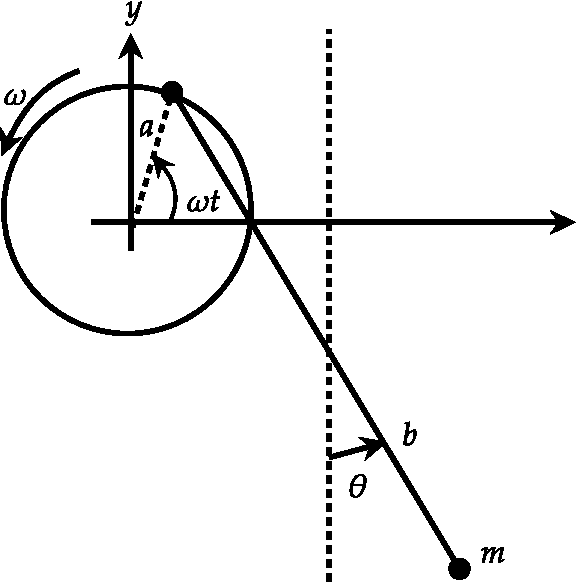
\includegraphics[height=5.5cm,width=5.5cm]{Assignment-HE-05}
	\end{figure}
	\begin{answer}
		\begin{align*}
		\intertext{(a) We choose the origin of our coordinate system to be at the center of the rotating rim. The Cartesian components of mass $m$ become}
		&\left.\begin{array}{l}x=a \cos \omega t+b \sin \theta \\ y=b \cos \theta-a \sin \omega t\end{array}\right\}
		\intertext{The velocities are}
		&\left.\begin{array}{l}\dot{x}=-a w \sin \omega t+b \dot{\theta} \cos \theta \\ \dot{y}=-a \omega \cos \omega t-b \dot{\theta} \sin \theta\end{array}\right\}
		\intertext{Taking the time derivative once again gives the acceleration:}
		\ddot{x}&=-a \omega^{2} \cos \omega t+b\left(\ddot{\theta} \cos \theta-\dot{\theta}^{2} \sin \theta\right)\\
		\ddot{y}&=+a \omega^{2} \sin \omega t-b\left(\ddot{\theta} \sin \theta+\dot{\theta}^{2} \cos \theta\right)
		\intertext{(b) It should now be clear that the single generalized coordinate is $\theta$. The kinetic and potential energies are}
	T &=\frac{1}{2} m\left(\dot{x}^{2}+\dot{y}^{2}\right) \\
	 U &=-m g y \\
	 \text{where }U&=0\text{ at }y=0.
	 \intertext{The Lagrangian of a system is given by}
	 L&=T-U=\frac{m}{2}\left[a^{2} \omega^{2}+b^{2} \dot{\theta}^{2}+2 b \dot{\theta} a \omega \sin (\theta-\omega t)\right]+m g(b \cos \theta-a \sin \omega t)
	 \intertext{(c) The derivatives for the Lagrange equation of motion for $\theta$ are}
	 \frac{d}{d t} \frac{\partial L}{\partial \dot{\theta}}&=m b^{2} \ddot{\theta}+m b a \omega(\dot{\theta}-\omega) \cos (\theta-\omega t)\\
	 \frac{\partial L}{\partial \theta}&=m b \dot{\theta} a \omega \cos (\theta-\omega t)-m g b \sin \theta
	 \intertext{which results in the equation of motion (after solving for $\ddot{\theta}$ )}
	 \ddot{\theta}&=\frac{\omega^{2} a}{b} \cos (\theta-\omega t)-\frac{g}{b} \sin \theta
		\end{align*}
	\end{answer}
	\item $\left. \right. $
	  \begin{figure}[H]
		\centering
		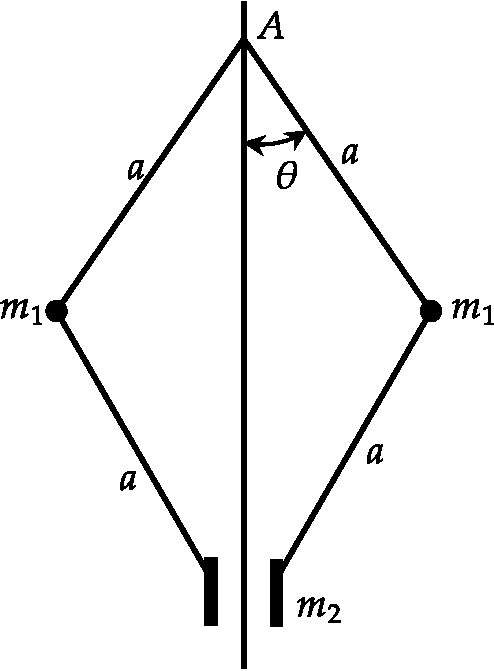
\includegraphics[height=6cm,width=3.6cm]{Assignment-HE-06}
	\end{figure}
	\begin{answer}
		\begin{align*}
		\text{(a) }&r_{1}=a, r_{2}=a, \theta_{1}=\theta_{2}=\theta, \quad \phi_{3}=0, \quad \theta_{3}=0, \quad r_{3}=2 a \cos \theta, \quad \phi_{1}=\phi_{2}+c\\
		&\text{Degree of freedom }=3 \times 3-7=2\\
	\text{	(b) }&L=m_{1} a^{2}\left(\dot{\theta}^{2}+\omega^{2} \sin ^{2} \theta\right)+2 m_{2} a^{2} \dot{\theta}^{2} \sin ^{2} \theta+2\left(m_{1}+m_{2}\right) g a \cos \theta\\
		\text{(c) }&\frac{d}{d t}\left(\frac{\partial L}{\partial \dot{\theta}}\right)-\frac{\partial L}{\partial \theta}=0\\
		&\frac{d}{d t}\left(2 m_{1} a^{2} \dot{\theta}+4 m_{2} a^{2} \dot{\theta} \sin ^{2} \theta\right)-m_{1} a^{2} \omega^{2} 2 \sin \theta \cos \theta-2 m_{2} a^{2} \dot{\theta}^{2} 2 \sin \theta \cos \theta+2\left(m_{1}+m_{2}\right) g a \sin \theta=0\\
		&\Rightarrow\left(2 m_{1} a^{2}+4 m_{2} a^{2} \sin ^{2} \theta\right) \ddot{\theta}+2 m_{2} a^{2} \sin 2 \theta \dot{\theta}^{2}-m_{1} a^{2} \omega^{2} \sin 2 \theta+2\left(m_{1}+m_{2}\right) g a \sin \theta=0\\
	\text{	(d) }&H=\sum \dot{\theta} p_{\theta}-L\\
	&\frac{\partial L}{\partial \dot{\theta}}=p_{\theta}=2 m_{1} a^{2} \dot{\theta}+4 m_{2} a^{2} \dot{\theta} \sin ^{2} \theta \Rightarrow \dot{\theta}=\frac{p_{\theta}}{2 m_{1} a^{2}+4 m_{2} a^{2} \sin ^{2} \theta}\\
	H&=\frac{p_{\theta}^{2}}{4 m a^{2}+\theta m_{2} a^{2} \sin ^{2} \theta}-m_{1} a^{2} \omega^{2} \sin ^{2} \theta-2\left(m_{1}+m_{2}\right) g a \cos \theta
		\end{align*}
	\end{answer}
	\item $\left. \right. $
	 \begin{figure}[H]
		\centering
		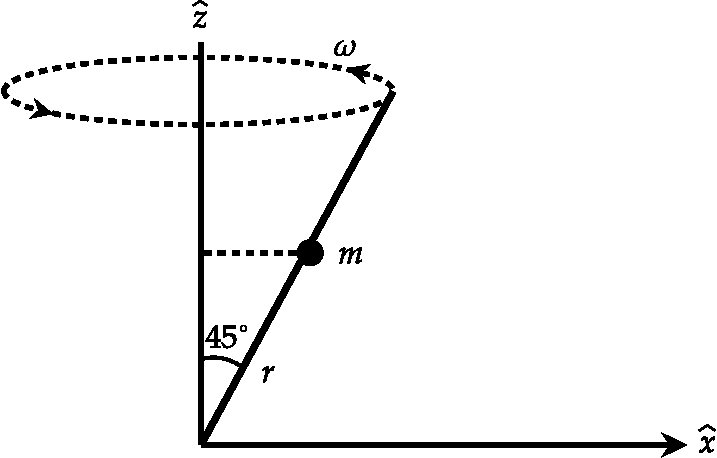
\includegraphics[height=4.5cm,width=6.5cm]{Assignment-HE-07}
	\end{figure}
	\begin{answer}
		\begin{align*}
		L&=\frac{1}{2} m\left(\dot{r}^{2}+r^{2} \dot{\theta}^{2}+r^{2} \sin ^{2} \theta \dot{\phi}^{2}\right)-m g r \cos \theta\\
		\text{equation of constrain is }\theta&=\frac{\pi}{4}\text{ and it is given }\dot{\phi}=\omega\\
		L&=\frac{1}{2} m\left(\dot{r}^{2}+\frac{1}{2} r^{2} \omega^{2}\right)-\frac{1}{\sqrt{2}} m g r\\
	\text{	the momentum conjugate to $r$ is }p_{r}&=\frac{\partial L}{\partial \dot{r}} \quad \Rightarrow p_{r}=m \dot{r}
		\end{align*}
	\end{answer}
		\item $\left. \right. $
		  \begin{figure}[H]
			\centering
			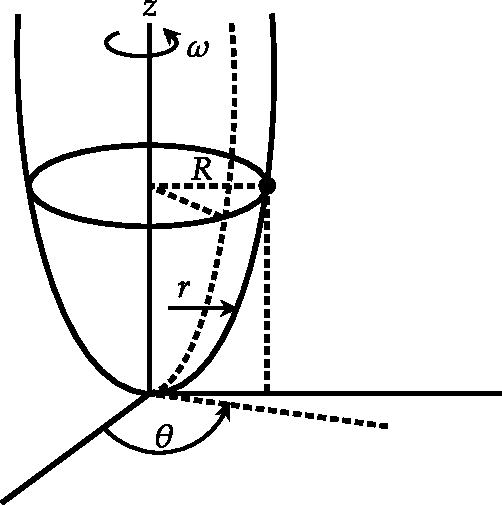
\includegraphics[height=6cm,width=5.2cm]{Assignment-HE-08}
		\end{figure}
	\begin{answer}
		\begin{align}
		\intertext{Because the problem has cylindrical symmetry, we choose $r, \theta$ and $z$ as the generalized coordinates. The kinetic energy of the bead is}
		T&=\frac{m}{2}\left[\dot{r}^{2}+\dot{z}^{2}+(r \dot{\theta})^{2}\right]\notag\\
	\text{	If we choose }U=0\text{ at }z&=0\text{, the potential energy term is}\notag\\
	U&=m g z\notag
	\intertext{But $r, z$ and $\theta$ are not independent. The equation of constraint for the parabola is}
	z&=c r^{2} \Rightarrow \dot{z}=2 c \dot{r} r\notag
	\intertext{We also have an explicit time dependence of the angular rotation}\notag
	\theta&=\omega t \Rightarrow \dot{\theta}=\omega\notag
	\intertext{We can now construct the Lagrangian as being dependent only on $r$, because there is no direct $\theta$ dependence.}
	L&=T-U=\frac{m}{2}\left(\dot{r}^{2}+4 c^{2} r^{2} \dot{r}^{2}+r^{2} \omega^{2}\right)-m g c r^{2}\notag
	\intertext{The problem stated that the bead moved in a circle of radius $R$. The reader might be tempted at this point to let $r=R=$ constant and $\dot{r}=0$. It would be a mistake to do this now in the Lagrangian. First, we should find the equation of motion for the variable $r$ and then let $r=R$ as a condition of the particular motion. This determines the particular value of $c$ needed for $r=R$.}\notag
	\frac{\partial L}{\partial \dot{r}}&=\frac{m}{2}\left(2 \dot{r}+8 c^{2} r^{2} \dot{r}\right), \frac{d}{d t} \frac{\partial L}{\partial \dot{r}}=\frac{m}{2}\left(2 \ddot{r}+16 c^{2} r \dot{r}^{2}+8 c^{2} r^{2} \ddot{r}\right)\notag\\
	\frac{\partial L}{\partial \dot{r}}&=m\left(4 c^{2} r \dot{r}^{2}+r \omega^{2}-2 g c r\right)\notag
	\intertext{Lagrange's equation of motion becomes}\notag\\
	\ddot{r}\left(1+4 c^{2} r^{2}\right)&+\dot{r}^{2}\left(4 c^{2} r\right)+r\left(2 g c-\omega^{2}\right)=0\label{HE-01}
	\intertext{which is a complicated result. If, however, the bead rotates with $r=R=$ constant, then $\dot{r}=\ddot{r}=0$ and equation (\ref{HE-01}) becomes}
	R\left(2 g c-\omega^{2}\right)&=0 \Rightarrow \omega=\sqrt{2 g c}\notag
		\end{align}
	\end{answer}
\end{enumerate}
\begin{abox}
	Assignment solution-2
\end{abox}
\begin{enumerate}
	\item $\left. \right. $
\begin{answer}
	\begin{align*}
	\text{Poisson bracket }\left[p_{x}-3 y, H\right]&=0 and \left[p_{y}+2 y, H\right]=0\\
	p_{y}(b-3)+x\left(3 b-b^{2}\right)&=0\text{ and }p_{x}(a+2)-y\left(2 a+a^{2}\right)=0\\
	\Rightarrow a&=-2, b=3
	\end{align*}
\end{answer} 
	\item $\left. \right. $
	\begin{answer}
		\begin{align*}
		H&=\sum \dot{q} p-L\text{ where }L=\frac{1}{2} m \dot{q}^{2}-\frac{1}{2} \lambda q \dot{q}^{2}\\
		\frac{\partial L}{\partial \dot{q}}&=p=m \dot{q}-\lambda q \dot{q} \Rightarrow p=\dot{q}(m-\lambda q) \Rightarrow \dot{q}=\frac{p}{m-\lambda q}\\
		\Rightarrow H&=\dot{q} p-L=\frac{p^{2}}{(m-\lambda q)}-\frac{1}{2} m \frac{\left(p^{2}\right)}{(m-\lambda q)^{2}}+\frac{\lambda}{2} q \cdot \frac{p^{2}}{(m-\lambda q)^{2}}\\
		\Rightarrow H&=\frac{p^{2}}{(m-\lambda q)}-\frac{p^{2}}{2(m-\lambda q)^{2}}(m-\lambda q)=\frac{p^{2}}{(m-\lambda q)}-\frac{p^{2}}{2(m-\lambda q)}\\
		\Rightarrow H&=\frac{p^{2}}{2(m-\lambda q)}
		\end{align*}
	\end{answer}
	\item $\left. \right. $
	\begin{answer}
		\begin{align*}
	\text{	(a) }\left\{C_{1}, C_{2}\right\}&=\left\{x_{2} p_{3}+x_{3} p_{2}, x_{1} p_{2}-x_{2} p_{1}\right\}\\
		\left\{C_{1}, C_{2}\right\} &=\left\{x_{2} p_{3}, x_{1} p_{2}\right\}-\left\{x_{2} p_{3}, x_{2} p_{1}\right\}+\left\{x_{3} p_{2}, x_{1} p_{2}\right\}-\left\{x_{3} p_{2}, x_{2} p_{1}\right\} \\
		&=x_{1}\left\{x_{2}, p_{2}\right\} p_{3}+0+0-x_{3}\left\{p_{2}, x_{2}\right\} p_{1}\\
		\Rightarrow\left\{C_{1}, C_{2}\right\}&=x_{1} p_{3}+x_{3} p_{1}\\
		\text{(b) }\left\{C_{1}, C_{2}\right\}&=C_{3}
		\end{align*}
	\end{answer}
	\item $\left. \right. $
\begin{answer}
	\begin{align*}
	\text{If $u$ is conserve then }\frac{d u}{d t}&=[u, H]+\frac{\partial u}{\partial t}=0 \Rightarrow \frac{d u}{d t}=\frac{\partial u}{\partial x} \cdot \frac{\partial H}{\partial p}-\frac{\partial u}{\partial p} \cdot \frac{\partial H}{\partial x}+\frac{\partial u}{\partial t}\\
	\Rightarrow \frac{d u}{d t}&=\frac{i m \omega}{p+i m \omega x} \cdot \frac{p}{m}-\frac{1}{p+i m \omega x} \cdot m \omega^{2} x-i \omega\\
	&=\frac{i \omega p}{p+i m \omega x}-\frac{m \omega^{2} x}{p+i m \omega x}-i \omega=\frac{i \omega(p+i m \omega x)}{p+i m \omega x}-i \omega=0
	\intertext{So $u$ is conserve during the motion}
	\end{align*}
\end{answer}
	\item $\left. \right. $
\begin{answer}
	\begin{align*}
	\intertext{(a) Solving Hamiltonian equation of motion}
	\frac{\partial H}{\partial x}&=-\dot{p}_{x} \Rightarrow p_{x}-x=-\dot{p}_{x}\text{ and }\frac{\partial H}{\partial y}=-\dot{p}_{y} \Rightarrow-p_{y}+y=-\dot{p}_{y}\\
	\frac{\partial H}{\partial p_{x}}&=\dot{x} \Rightarrow x=\dot{x}\text{ and } \frac{\partial H}{\partial p_{y}}=\dot{y} \Rightarrow-y=\dot{y}
	\intertext{(b) After solving these four differential equation and eliminating time $t$ and using boundary condition one will get $\Rightarrow x \propto \frac{1}{y}$ and $p_{x} \propto \frac{1}{p_{y}}$}
	\end{align*}
\end{answer}
	\item $\left. \right. $
\begin{answer}
	\begin{align}
	H&=\frac{p^{2}}{2 m}+\frac{1}{2} m \omega^{2} q^{2}, \quad F=F_{1}(q, Q)=-\frac{Q}{q}\notag\\
	\Rightarrow \frac{\partial F_{1}}{\partial q}&=p \Rightarrow \frac{Q}{q^{2}}=p\label{HE02}\\
	\Rightarrow \frac{\partial F_{1}}{\partial Q}&=-P \Rightarrow-\frac{1}{q}=-P \Rightarrow q=\frac{1}{P}\label{HE-03}
	\intertext{From equation (\ref{HE02}) and (\ref{HE-03}) $\Rightarrow p=Q P^{2}$	$
		\quad \because q=\frac{1}{P}	$}\notag
	H&=\frac{p^{2}}{2 m}-\frac{1}{2} m \omega^{2} q^{2}=\frac{Q^{2} P^{4}}{2 m}-\frac{1}{2} m \omega^{2}\left(\frac{1}{P^{2}}\right)=\frac{1}{2 m} Q^{2} P^{4}-\frac{1}{2} m \omega^{2} P^{-2}\notag
	\end{align}
\end{answer}
	\item $\left. \right. $
\begin{answer}
	\begin{align*}
		H&=\frac{p_{x}^{2}}{2 m}+\frac{p_{y}^{2}}{2 m}+\frac{1}{2} m \omega^{2}\left(x^{2}+y^{2}\right) \quad S_{1}=\frac{1}{2}\left(x p_{y}-y p_{x}\right)\\
		\text{(a) }&\left[S_{1}, H\right]=0\\
		&\Rightarrow \frac{\partial S_{1}}{\partial x} \frac{\partial H}{\partial p_{x}}-\frac{\partial S_{1}}{\partial p_{x}} \frac{\partial H}{\partial x}+\frac{\partial S_{1}}{\partial y} \frac{\partial H}{\partial p_{y}}-\frac{\partial S_{1}}{\partial p_{y}} \cdot \frac{\partial H}{\partial y} \\
		&\Rightarrow \frac{p_{y}}{2} \cdot \frac{p_{x}}{m}-\left(-\frac{y}{2}\right) \cdot m \omega^{2} x+\frac{1}{2}\left(-p_{x}\right) \cdot \frac{p_{y}}{m}-\frac{1}{2}(x) \cdot m \omega^{2} y=0\\
		\text{(b) }&\left[S_{2}, H\right]=0\hspace{2cm}
		S_{2}=\frac{1}{2 m \omega}\left(p_{x} p_{y}+m^{2} \omega^{2} x y\right)\\
		&\Rightarrow \quad \frac{\partial S_{2}}{\partial x} \frac{\partial H}{\partial p_{x}}-\frac{\partial S_{2}}{\partial p_{x}} \frac{\partial H}{\partial x}+\frac{\partial S_{2}}{\partial y} \frac{\partial H}{\partial p_{y}}-\frac{\partial S_{2}}{\partial p_{y}} \frac{\partial H}{\partial y}\\
		&\Rightarrow \quad \frac{1}{2 m \omega}\left(m^{2} \omega^{2} y\right)\left(\frac{p_{x}}{m}\right)-\frac{p_{y}}{2 m \omega} \cdot\left(m \omega^{2} x\right)+\frac{1}{2 m \omega} m^{2} \omega^{2} x \cdot \frac{p_{y}}{m}-\frac{p_{x}}{2 m \omega} \cdot m \omega^{2} y=0\\
		\text{(c) }&\left[S_{3}, H\right]=0\\
		&\frac{\partial S_{3}}{\partial x} \frac{\partial H}{\partial p_{x}}-\frac{\partial S_{3}}{\partial p_{x}} \frac{\partial H}{\partial x}+\frac{\partial S_{3}}{\partial y} \frac{\partial H}{\partial p_{y}}-\frac{\partial S_{3}}{\partial p_{y}} \cdot \frac{\partial H}{\partial y} \\
		&\Rightarrow \frac{1}{4 m \omega} \times m^{2} \omega^{2}(-2 x) \cdot \frac{p_{x}}{m}-\frac{1}{4 m \omega} \times 2 p_{x} \cdot m \omega^{2} x+\frac{m^{2} \omega^{2}}{4 m \omega} \times 2 y \cdot \frac{p_{y}}{m}-\frac{1}{4 m \omega}\left(-2 p_{y} \cdot m \omega^{2} y\right) \\
		&\Rightarrow \frac{-p_{x} x \omega}{2}-\frac{p_{x} \omega x}{2}+\frac{p_{y} \cdot y \omega}{2}+\frac{p_{y} y \omega}{2} \neq 0
	\end{align*}
\end{answer}
	\item $\left. \right. $
\begin{answer}
	\begin{align*}
	Q&=\log \left(1+q^{\frac{1}{2}} \cos p\right)\\
	P&=2\left(1+q^{\frac{1}{2}} \cos p\right) q^{\frac{1}{2}} \sin p \Rightarrow 2 q^{\frac{1}{2}} \sin p+q \sin 2 p\\
\text{	(a) }&\text{For canonical transformation: }\frac{\partial Q}{\partial q} \cdot \frac{\partial P}{\partial p}-\frac{\partial Q}{\partial p} \cdot \frac{\partial P}{\partial q}=1\\
	&\Rightarrow \frac{\partial Q}{\partial q}=\frac{1}{\left(1+q^{\frac{1}{2}} \cos p\right)} \times \frac{1}{2} q^{-\frac{1}{2}} \cos p, \frac{\partial Q}{\partial p}=\frac{q^{\frac{1}{2}}(-\sin p)}{\left(1+q^{\frac{1}{2}} \cos p\right)}\\
	\frac{\partial P}{\partial p}&=2 q^{\frac{1}{2}} \cos p+2 q \cos 2 p, \frac{\partial P}{\partial q}=2 \times \frac{1}{2} q^{-\frac{1}{2}} \sin p+\sin 2 p\\
	&\Rightarrow \frac{\cos p}{2\left(1+q^{\frac{1}{2}} \cos p\right) q^{\frac{1}{2}}} \cdot 2\left(q^{\frac{1}{2}} \cos p+q \cos 2 p\right)-\frac{\left(-q^{\frac{1}{2}} \sin p\right)}{\left(1+q^{\frac{1}{2}} \cos p\right)} \times\left(q^{-\frac{1}{2}} \sin p+\sin 2 p\right)=1\\
	\text{(b) }F_{3}&=F_{3}(p, Q, t)\\
	\frac{\partial F_{3}}{\partial p}&=-q, \quad \frac{\partial F_{3}}{\partial Q}=-P \\
	Q&=\log \left(1+q^{1 / 2} \cos p\right) \Rightarrow e^{Q}=1+q^{1 / 2} \cos p\\
	\frac{e^{Q}-1}{\cos p}&=q^{1 / 2} \Rightarrow q=\left(\frac{e^{Q}-1}{\cos p}\right)^{2}\\
	P&=2\left(1+q^{1 / 2} \cos p\right) q^{1 / 2} \sin p \Rightarrow P=2 e^{Q} q^{1 / 2} \sin p \Rightarrow 2 e^{Q}\left(e^{Q}-1\right) \tan p\\
	\frac{\partial F_{3}}{\partial p}&=-q=-\frac{\left(e^{Q}-1\right)^{2}}{\cos ^{2} p} \Rightarrow F_{3}=-\int\left(e^{Q}-1\right)^{2} \sec ^{2} p d p
	\end{align*}
	\begin{align}
	F_{3}&=-\left(e^{Q}-1\right)^{2} \tan p+f_{1}(Q)\label{HE-04}\\
	\frac{\partial F_{3}}{\partial Q}&=-P=-2\left(e^{2 Q}-e^{Q}\right) \tan p\notag\\
	F_{3}&=-2\left(\frac{1}{2} e^{2 Q}-e^{Q}\right) \tan p+f_{2}(p)=-\left(e^{Q}-1\right)^{2} \tan p+\tan p+f_{2}(p) \label{HE-05}
\intertext{	Equating $\ref{HE-04}$ and $\ref{HE-05}$}
	f_{1}(Q)&=0, \quad f_{2}(p)=-\tan p\notag\\
	\text{So }F_{3}&=-\left(e^{Q}-1\right)^{2} \tan p \notag
	\end{align}
\end{answer}
	\item $\left. \right. $
\begin{answer}
	\begin{align*}
	\frac{\partial Q_{1}}{\partial q_{1}} \frac{\partial P_{1}}{\partial p_{1}}&-\frac{\partial Q_{1}}{\partial p_{1}} \frac{\partial P_{1}}{\partial q_{1}}+\frac{\partial Q_{1}}{\partial q_{2}} \frac{\partial P_{1}}{\partial p_{2}}-\frac{\partial Q_{1}}{\partial p_{2}} \frac{\partial P_{1}}{\partial q_{2}}=1 \times 1-0=1\\
	\text{and }&\frac{\partial Q_{1}}{\partial q_{1}} \frac{\partial P_{1}}{\partial p_{1}}-\frac{\partial Q_{1}}{\partial p_{1}} \frac{\partial P_{1}}{\partial q_{1}}+\frac{\partial Q_{2}}{\partial q_{2}} \frac{\partial P_{2}}{\partial p_{2}}-\frac{\partial Q}{\partial p_{2}} \frac{\partial P_{2}}{\partial q_{2}}=0-(-1)=1
	\end{align*}
\end{answer}
	\item $\left. \right. $
\begin{answer}$\left. \right. $
		\begin{figure}[H]
		\centering
		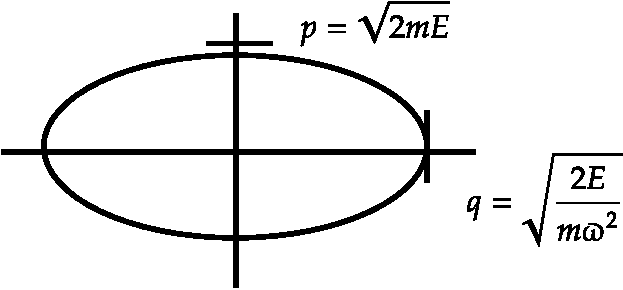
\includegraphics[height=2.5cm,width=5cm]{Assignment-HE-13.pdf}
	\end{figure}
	\begin{align*}
	\text{(A)\quad (a)\quad }H&=\frac{1}{2 m}\left[p^{2}+m^{2} \omega^{2} q^{2}\right]\\
	\frac{\partial H}{\partial p}&=\dot{q} \Rightarrow \frac{p}{m}=\dot{q} \Rightarrow p=m \dot{q}\\
	\frac{\partial H}{d q}&=-\dot{p} \Rightarrow m \omega^{2} q=-\dot{p}\\
	-m \omega^{2} q&=m \ddot{q}\\\
	\ddot{q}+\omega^{2} q&=0\\
	q&=A \cos \omega t+B \sin \omega t
	\end{align*}
		\begin{figure}[H]
		\centering
		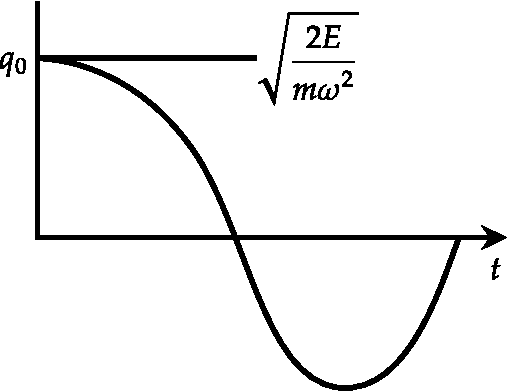
\includegraphics[height=3cm,width=4cm]{Assignment-HE-14.pdf}
	\end{figure}
	\begin{align*}
	\text{(b) \quad}&\frac{p^{2}}{(\sqrt{2 m E})^{2}}+\frac{q^{2}}{\left(\sqrt{\frac{2 E}{m \omega^{2}}}\right)^{2}}=1\\
	\text{(c) \quad}&\text{ With initial condition, when }t=0, q=q_{0}\text{ and } \dot{q}=0\text{ at }t=0\\
	\text{Then, }q_{0}&=A\text{ and }q=q_{0} \cos \omega t\\
	\text{(d) }\quad p&=m \dot{q}\\
	p&=-q_{0} \omega m \sin \omega t
	\end{align*}
		\begin{figure}[H]
		\centering
		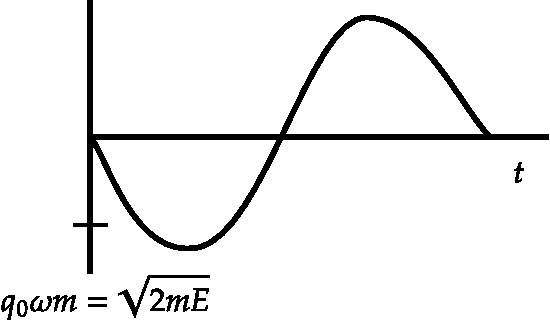
\includegraphics[height=2.8cm,width=4.5cm]{Assignment-HE-12.pdf}
	\end{figure}
	\begin{align*}
\text{	(B)\quad  (a)\quad }F_{1}&=\frac{m \omega q^{2}}{2} \cot Q, \frac{\partial F_{1}}{\partial q}=p, \frac{\partial F_{1}}{\partial Q}=-P\\
m \omega q \cdot \cot Q&=p,-\frac{m \omega q^{2}}{2} \operatorname{cosec} Q=-P\\
q^{2}&=\frac{2 P}{m \omega} \frac{1}{\operatorname{cosec}{ }^{2} Q}\\
q&=\sqrt{\frac{2 P}{m \omega}} \sin Q, p=m \omega \sqrt{\frac{2 P}{m \omega}} \cot Q \sin Q\\
p&=\sqrt{2 m P \omega} \cos Q\\
\text{(b) }\quad H&=\frac{p^{2}}{2 m}+\frac{1}{2} m \omega^{2} q^{2}\\
K&=H+\frac{\partial F_{1}}{\partial t} \Rightarrow \frac{\partial F_{1}}{\partial t}=0, K=H=\frac{1}{2 m}(\sqrt{2 P m \omega} \cos Q)^{2}+\frac{1}{2} m \omega^{2}\left(\sqrt{\frac{2 P}{m \omega}}\right)^{2} \sin ^{2} Q\\
K&=\omega P\\
\text{(c)\quad}&
\frac{\partial K}{\partial Q}=-\dot{P} \Rightarrow \dot{P}=0, \frac{d P}{d t}=0, P=c\\
\frac{\partial K}{\partial P}&=\dot{Q}=\omega, Q=\omega t+\alpha\text{ where } \alpha\text{ is constant, can be find with initial condition}
	\end{align*}
	\begin{figure}[H]
		\centering
		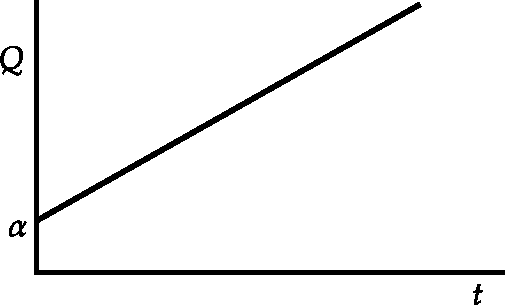
\includegraphics[height=2.8cm,width=4.5cm]{Assignment-HE-09.pdf}
	\end{figure}
 \begin{tasks}(1)
	\task[\text{(d)}] 
	\begin{figure}[H]
		\centering
		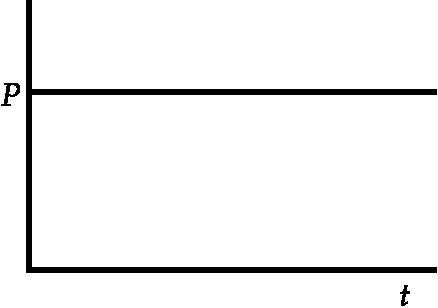
\includegraphics[height=2.8cm,width=4.5cm]{Assignment-HE-10.pdf}
	\end{figure}where $P=\frac{E}{\omega}$
	\task[\text{(e)}] 
		\begin{figure}[H]
		\centering
		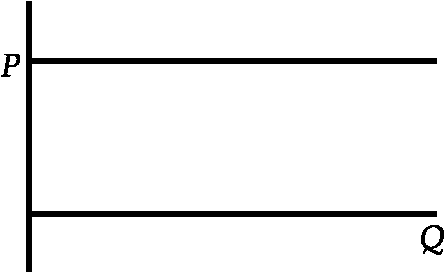
\includegraphics[height=2.8cm,width=4.5cm]{Assignment-HE-11.pdf}
	\end{figure}
\end{tasks}
\end{answer}
	\item $\left. \right. $
	\begin{answer}
		\begin{align*}
		F_{2}&=q^{2} P\\
		\frac{\partial F_{2}}{\partial q}&=2 q P=p, \frac{\partial F_{2}}{\partial P}=q^{2}=Q, q=\sqrt{Q}, p=2 \sqrt{Q} P\\
		K&=\frac{p^{2}}{2 \alpha q^{2}}+\frac{\beta \cdot q^{4}}{4}=\frac{4 Q P^{2}}{2 \alpha Q}+\frac{\beta Q^{2}}{4} \Rightarrow K=\frac{2 P^{2}}{\alpha}+\frac{\beta Q^{2}}{4}\\
		\frac{\partial K}{\partial P}&=\dot{Q} \Rightarrow \frac{4 P}{\alpha}=\dot{Q}\\
		\frac{\partial K}{\partial Q}&=-\dot{P} \Rightarrow \frac{\beta Q}{2}=-\dot{P}
		\end{align*}
	\end{answer}
	\item $\left. \right. $
	\begin{answer}
		\begin{align*}
		\text{(a) }L&=\frac{1}{2} m \dot{x}^{2}+m\left(\dot{y}^{2}+\dot{z}^{2}\right)-\frac{1}{2} k x^{2}-\frac{1}{2} k(y+z)^{2}\\
		H&=\frac{p_{x}^{2}}{2 m}+\frac{p_{y}^{2}}{4 m}+\frac{p_{z}^{2}}{4 m}+\frac{1}{2} k x^{2}+\frac{1}{2} k(y+z)^{2}\\
		\text{(b) }\quad L_{z}^=x p_{y}-y p_{x}\\
		\frac{d L_{z}}{d t}&=\left[L_{z} H\right]+\frac{\partial L_{z}}{\partial t}, \frac{\partial L_{z}}{\partial t}=0\\
		\left[L_{z}, H\right]&=\left[x p_{y}-y p_{x}, H\right]=x\left[p_{y}, H\right]+[x, H] p_{y}-y\left[p_{x}, H\right]-[y, H] p_{x} \\
		&=x\left[p_{y}, \frac{1}{2} k(y+z)^{2}\right]+\left[x, \frac{p_{x}^{2}}{2 m}\right] p_{y}-y\left[p_{x}, \frac{1}{2} k x^{2}\right]-\left[y, \frac{p_{y}^{2}}{4 m}\right] p_{x}\\
		&=x(-k(y+z))+\frac{p_{x} p_{y}}{m}+k y x-\frac{p_{x} p_{y}}{2 m}\\
		\left[L_{z}, H\right]&=\frac{p_{y} p_{x}}{2 m}-k x z, \frac{d L_{z}}{d t}=\frac{p_{x} p_{y}}{2 m}-k x z \\
		\text{(c) }\quad\left[L_{x}, H\right]&=\left[y p_{z}-z p_{y}, H\right]=\left[y p_{z}, H\right]-\left[z p_{y}, H\right]\\
		&=[y, H] p_{z}+y\left[p_{z}, H\right]-[z, H] p_{y}-z\left[p_{y}, H\right]\\
		&=\left[y, \frac{p_{y}^{2}}{4 m}\right] p_{z}+y\left[p_{z}, \frac{1}{2} k(y+z)^{2}\right]-\left[z, \frac{p_{z}^{2}}{4 m}\right] p_{y}-z\left[p_{y}, \frac{1}{2} k(y+z)^{2}\right]\\
		&=\frac{p_{y}}{2 m} p_{z}+y[-k(y+z)]-\frac{p_{z}}{2 m} p_{y}+k z(y+z)=-k y^{2}-k z y+k z y+k z^{2}\\
		\left[L_{x}, H\right]&=k\left[z^{2}-y^{2}\right], \frac{d L_{x}}{d t}=k\left[z^{2}-y^{2}\right] \\
		\text{(d) }\quad \frac{d L_{y}}{d t}&=-\frac{p_{x} p_{z}}{2 m}+k x y\\
	\text{	(e)\quad }
		\frac{\partial H}{\partial x}&=-\dot{p}_{x}, k x=-\dot{p}_{x}=\frac{-d p_{x}}{d t} \Rightarrow \frac{d p_{x}}{d t}=-k x\\
		\frac{\partial H}{\partial y}&=-\dot{p}_{y}, \frac{2 k}{2}(y+z)=-\dot{p}_{y}, \frac{d p_{y}}{d t}=-k(y+z)
		\end{align*}
	\end{answer}
\end{enumerate}